
\section{Additional categorical validation on Optdigits}
\label{app:bandit}

This appendix records an auxiliary finite-population check of the theoretical
mechanism. The experiment is a one-step contextual bandit with ten categorical
actions. Unlike the Gaussian example in Section~\ref{sec:gaussian-example},
its moments are obtained by exact enumeration over a real dataset rather than
closed-form integration. It is not needed to establish the two crossovers in
Section~\ref{sec:gaussian-example}.

\subsection{Auxiliary results}
\label{app:optdigits-results}

We convert Optdigits into a one-step contextual bandit
\citep{alpaydin1998optdigits}. Each image is a context, the action is a digit,
and the reward is one only for the correct class. The policy is a linear
softmax classifier. Each policy iteration draws 320 contexts from a frozen
rollout policy and uses the resulting observations in eight minibatches of 40.
The construction and exact finite-population quantities are given below.

We first freeze 30 policy pairs across the observed population-ESS range. At
each pair, enumeration of the finite context--action space gives the exact MSE
of the IS and PPO estimators for a minibatch of 40. We also draw 80 independent
minibatches and apply the first 20 sampled directions with the globally valid
step size $\eta=0.17$. In the lowest-support bin, the median ESS is $0.190$ and
the IS and PPO MSEs are $1311421.7185$ and $1311421.1710$. PPO has lower MSE
at every state in this bin. In the highest-support bin, the corresponding MSEs
are $0.0633$ and $0.0617$, and PPO has lower MSE at only 20.0\% of states.

The error-to-signal boundary also predicts harmful sampled updates. For IS,
none of the 48 updates with realized squared error below the gradient signal is
harmful, whereas 8.7\% of the 552 updates above the boundary decrease the
population objective. The corresponding PPO rates are 0.0\% among 97 updates
below the boundary and 5.8\% among 503 updates above it.

\begin{figure}[htbp]
  \centering
  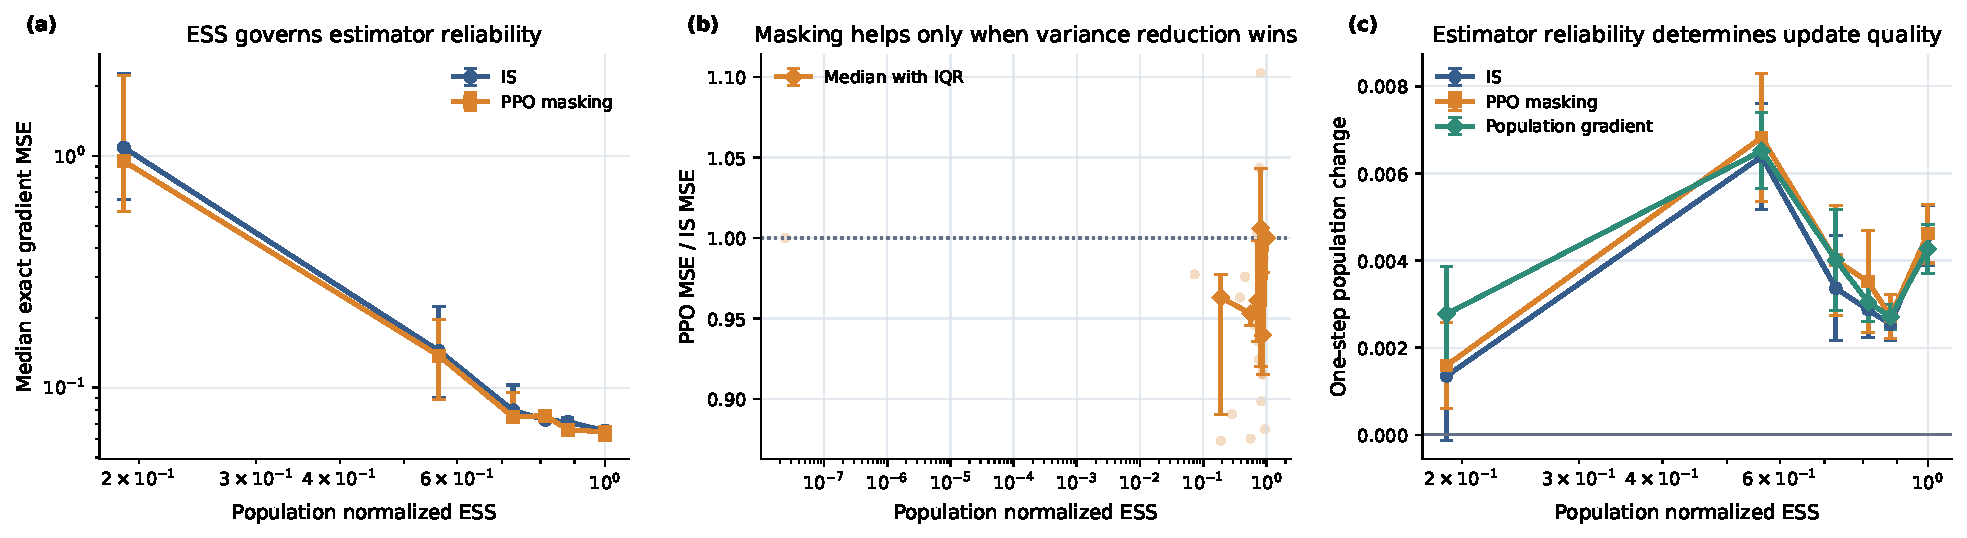
\includegraphics[width=\linewidth]{figures/optdigits_estimator_comparison.pdf}
  \caption{Auxiliary Optdigits comparison of IS and PPO. (a) Exact gradient
  MSE across population normalized ESS. (b) Harmful-update rate as realized
  squared gradient error crosses the population-gradient signal. (c) One-step
  population change under the globally valid step size.}
  \label{fig:optdigits-theory}
\end{figure}

A second deterministic path compares the two statewise oracles directly. At
$\rho=0.5577$, PPO has lower MSE, but its MSE reduction is smaller than the
retained-update requirement in
Equation~\eqref{eq:is-ppo-certificate-crossover}. IS therefore has the
stronger positive certificate. At $\rho=0.5489$, the inequality reverses and
the safe certificate oracle switches to PPO. PPO remains certified down to
$\rho=0.5363$, after which both certificates are nonpositive. This path is a
common-state diagnostic rather than a learning trajectory.

On the displayed low-support branch, a pairwise ESS threshold at
$\rho=0.54893$ matches all 490 interleaved evaluation states. Adding the null
choice gives an IS--PPO--no-update ESS rule that matches 489 of 490 states.
The complete path contains a small disconnected PPO interval, so the same
three-way rule has balanced accuracy $0.778$ and PPO recall $3/9$ over the full
path. This limitation is why the analytic Gaussian construction, rather than
Optdigits, carries the main-text oracle claim.

\begin{figure}[htbp]
  \centering
  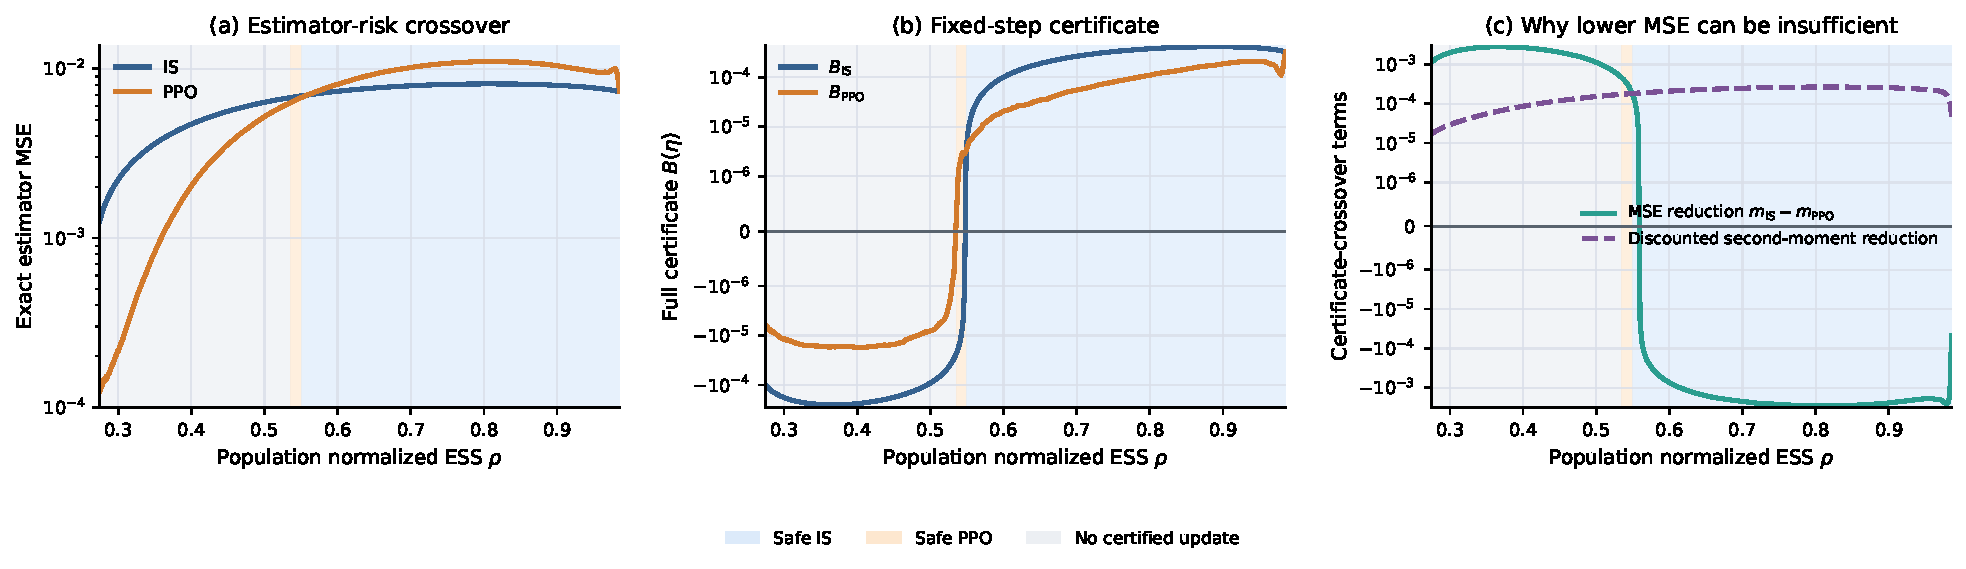
\includegraphics[width=\linewidth]{figures/optdigits_full_certificate.pdf}
  \caption{Auxiliary exact common-state Optdigits comparison for an iid
  minibatch of $N=320$. (a) MSE ordering changes before fixed-step ordering.
  (b) The safe certificate oracle selects IS, then PPO, and finally no update
  on the displayed low-support branch. (c) PPO has the stronger full
  certificate only when its MSE reduction exceeds the retained-update
  requirement.}
  \label{fig:optdigits-full-certificate}
\end{figure}

Finally, Figure~\ref{fig:optdigits-learning} reports a separate 40-update
learning curve with a fresh rollout every eight updates. Across 100 paired
replications, IS retains a small early advantage because support remains broad
enough for PPO masking to remove more useful signal than variance. Both methods
finish at population value $0.500$ to the reported precision. No oracle or ESS
gate is applied on this trajectory.

\begin{figure}[htbp]
  \centering
  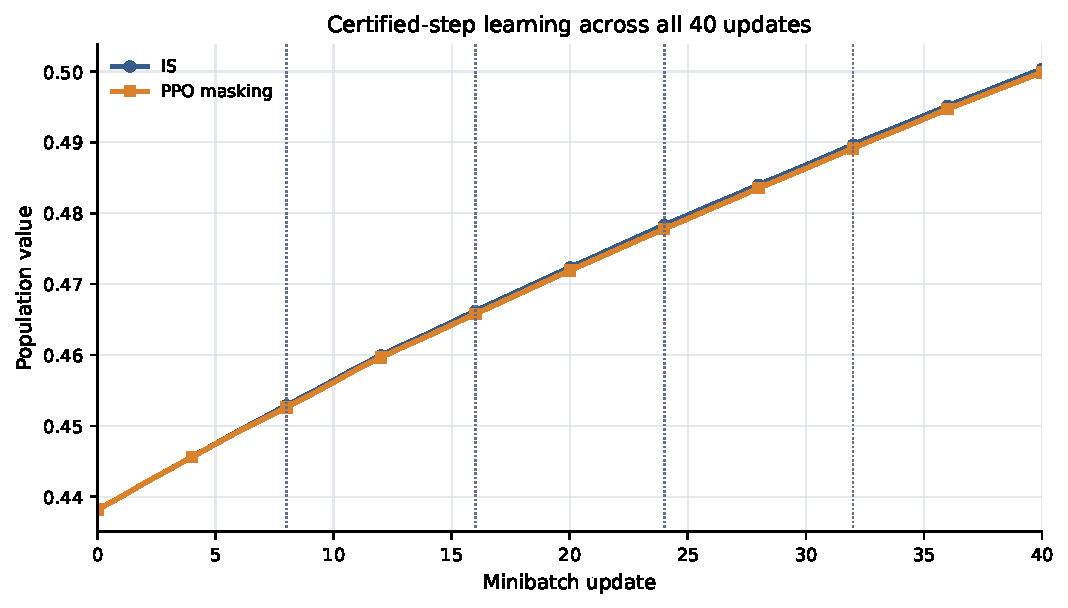
\includegraphics[width=0.72\linewidth]{figures/optdigits_certified_learning.pdf}
  \caption{Auxiliary Optdigits population value across 40 minibatch updates.
  Curves show means and 95\% confidence intervals over 100 paired replications.
  Dotted vertical lines mark collection of a fresh rollout.}
  \label{fig:optdigits-learning}
\end{figure}

\subsection{Finite population and policy}

Optdigits contains 5,620 labeled handwritten-digit images \citep{alpaydin1998optdigits}. We concatenate the supplied training and test files, divide each of the 64 pixel-count features by 16, and append an intercept. The resulting finite population is $\{(x_j,y_j)\}_{j=1}^M$ with $M=5{,}620$, $x_j\in\mathbb R^{65}$, and $y_j\in\{0,\ldots,9\}$. The original split is not used because the target is finite-population policy optimization rather than classification generalization.

The policy is a linear softmax model,
\begin{equation}
 \pi_\theta(a\mid x)
 =\frac{\exp(\theta_a^\top x)}{\sum_{c=0}^9\exp(\theta_c^\top x)},
 \qquad a\in\{0,\ldots,9\}.
 \label{eq:categorical-policy}
\end{equation}
The reward is $R(x_j,a)=\mathbf 1\{a=y_j\}$, so the exact population objective and gradient are
\begin{align}
 J(\theta)&=\frac1M\sum_{j=1}^M\pi_\theta(y_j\mid x_j),
 \label{eq:categorical-value}\\
 g(\theta)&=\frac1M\sum_{j=1}^M
 \pi_\theta(y_j\mid x_j)
 \{e_{y_j}-\pi_\theta(\cdot\mid x_j)\}x_j^\top.
 \label{eq:categorical-gradient}
\end{align}
Both quantities are evaluated by summing over all images. The policy is initialized by 400 full-population cross-entropy steps with step size $0.5$, after which the fitted weights are multiplied by $0.35$.

\subsection{A global smoothness certificate}
\label{app:optdigits-smoothness}

Let $p=\operatorname{softmax}(z)$ and $q=p_y$. The Hessian of one correct-class probability with respect to the logits is
\begin{equation}
 \nabla_z^2q
 =q\left[
 (e_y-p)(e_y-p)^\top-\{\operatorname{diag}(p)-pp^\top\}
 \right].
 \label{eq:categorical-logit-hessian}
\end{equation}
The categorical covariance satisfies $\|\operatorname{diag}(p)-pp^\top\|_{\mathrm{op}}\le1/2$, and $\|e_y-p\|_2^2\le2(1-q)^2$. Hence
\begin{equation}
 \|\nabla_z^2q\|_{\mathrm{op}}
 \le q\{2(1-q)^2+1/2\}
 \le1/2.
 \label{eq:categorical-logit-bound}
\end{equation}
For a perturbation $U$ of the softmax parameter matrix, Equation~\eqref{eq:categorical-logit-bound} gives
\begin{align}
 \left|\nabla^2J(\theta)[U,U]\right|
 &\le\frac{1}{2M}\sum_{j=1}^M\|Ux_j\|_2^2
 \nonumber\\
 &\le\frac12\lambda_{\max}\left(
 \frac1M\sum_{j=1}^Mx_jx_j^\top
 \right)\|U\|_F^2.
 \label{eq:categorical-smoothness-bound}
\end{align}
Thus a valid global smoothness constant is $\bar L=\tfrac12\lambda_{\max}(M^{-1}\sum_jx_jx_j^\top)$. For Optdigits, $\lambda_{\max}=11.549$, so $\bar L=5.775$ and $1/\bar L=0.173$. All evaluated updates use $\eta=0.17\le1/\bar L$.

\subsection{Sampling and gradient estimators}

At each policy iteration, we freeze the current policy as $Q$, draw 320 contexts independently and uniformly from the finite population, and sample one action from $Q(\cdot\mid x)$ for each context. Since the reward is exact class match, the state value under $Q$ is $Q(y\mid x)$. We use the detached exact baseline and set $A=R-Q(y\mid x)$. The 320 observations are randomly partitioned into eight minibatches of size $N=40$ and traversed once. The rollout is then discarded.

The IS estimator is
\begin{equation}
 \widehat g_{\mathrm{IS}}(\theta)
 =\frac1N\sum_{i=1}^N
 \frac{\pi_\theta(a_i\mid x_i)}{Q(a_i\mid x_i)}
 A_i\nabla_\theta\log\pi_\theta(a_i\mid x_i).
 \label{eq:categorical-is-gradient}
\end{equation}
The PPO estimator multiplies each sampled contribution by the standard advantage-dependent mask with radius $0.2$.

For $e\in\{\mathrm{IS},\mathrm{PPO}\}$, let $Z_e$ denote one gradient contribution. Since the context population and action space are finite, the exact conditional MSE is
\begin{equation}
 m_e(\theta,Q)
 =\left\|\E_Q[Z_e]-g(\theta)\right\|_2^2
 +\frac1N\E_Q\left\|Z_e-\E_Q[Z_e]\right\|_2^2.
 \label{eq:categorical-exact-risk}
\end{equation}
We calculate Equation~\eqref{eq:categorical-exact-risk} by summing over all $5{,}620\times10$ context-action pairs.

\subsection{Frozen-state estimator comparison}

To obtain policy pairs spanning a wide ESS range, we generate a separate state library from six policy iterations of the static IS and PPO updates under a stress step size. This trajectory is used only to define fixed pairs $(P_\theta,Q)$. No population-change result is computed using the stress step. We order the resulting pre-update states by exact population ESS,
\begin{equation}
 \rho(\theta,Q)
 =\left\{
 \frac1M\sum_{j=1}^M\sum_{a=0}^9
 \frac{\pi_\theta(a\mid x_j)^2}{Q(a\mid x_j)}
 \right\}^{-1},
 \label{eq:categorical-population-ess}
\end{equation}
and retain 30 approximately equally spaced states. At each state, the exact MSE uses minibatch size 40, and 80 independent minibatches estimate realized gradient error. The first 20 redraws receive the certified step $\eta=0.17$, after which the exact objective is recomputed.

\begin{table}[htbp]
\centering
\small
\caption{Optdigits estimator comparison across equal-count population-ESS bins. Exact MSE includes both squared bias and variance divided by 40. Harmful-update rates use the certified step size.}
\label{tab:categorical-ess-bins}
\begin{tabular}{rrrrr}
\toprule
Median ESS & IS MSE & PPO MSE & IS harmful (\%) & PPO harmful (\%) \\
\midrule
$0.190$ & $1311421.7185$ & $1311421.1710$ & $30.0$ & $12.0$ \\
$0.563$ & $0.1548$ & $0.1443$ & $7.0$ & $5.0$ \\
$0.728$ & $0.0959$ & $0.0921$ & $6.0$ & $2.0$ \\
$0.814$ & $0.0755$ & $0.0748$ & $4.0$ & $7.0$ \\
$0.879$ & $0.0721$ & $0.0683$ & $1.0$ & $3.0$ \\
$1.000$ & $0.0633$ & $0.0617$ & $0.0$ & $0.0$ \\
\bottomrule
\end{tabular}
\end{table}

\subsection{Common-state full-certificate comparison}

The full-certificate experiment is a separate deterministic construction. It
uses only the official training split, containing $3{,}823$ contexts. A linear
classifier $W_{\rm fit}$ is obtained with the same 400 full-population
cross-entropy steps as above. The frozen rollout and common-state path are
\begin{equation}
 Q=\pi_{0.2W_{\rm fit}},
 \qquad
 \theta(\lambda)=0.2W_{\rm fit}
 +\lambda(1.0-0.2)W_{\rm fit},
 \qquad \lambda\in[0,2.5].
 \label{eq:categorical-certificate-path}
\end{equation}
We evaluate 1,001 equally spaced values of $\lambda$. This path is chosen to
provide common policy states across a broad support range; it is not generated
by repeatedly applying either estimator.

For every state, we enumerate all $3{,}823\times10$ context--action pairs. This
gives the exact $g$, $\mu_u$, $s_u$, and $m_u$ for both IS and the
advantage-dependent PPO mask, with iid minibatch size $N=320$, where
$\mu_u:=\E[\widehat g_u]$, $s_u:=\E\|\widehat g_u\|_2^2$, and
$m_u:=\E\|\widehat g_u-g\|_2^2$. We then compute
\begin{equation}
 B_u(\eta)=\eta g^\top\mu_u-\frac{L\eta^2}{2}s_u,
 \qquad
 L=\frac12\lambda_{\max}\left(
 \frac1{3{,}823}\sum_jx_jx_j^\top
 \right)=5.801469,
 \label{eq:categorical-exact-full-certificate}
\end{equation}
using $\eta=0.17$ and PPO radius $0.2$. Thus $\eta L=0.986250<1$.
The estimator-risk oracle minimizes $m_u$, the forced certificate oracle
maximizes $B_u$, and the safe certificate oracle additionally includes a null
update with certificate zero and resolves nonpositive choices in favor of the
null update. All three are statewise definitions; none observes future values
or optimizes cumulative return.

For the path-specific ESS diagnostic, we restrict to $\lambda\ge0.05$, assign
alternating grid points to calibration and evaluation, and fit monotone ESS
cuts on the calibration points. This interleaved split checks interpolation
between adjacent states on the same deterministic path. It is deliberately not
described as validation on an independent trajectory. The complete path,
including the small disconnected high-ESS PPO interval, is retained in the
reported data artifact even though Figure~\ref{fig:optdigits-full-certificate}
focuses on the main low-support branch.

\subsection{Full certified learning curve}

The learning comparison uses five policy iterations and 100 paired replications. Each iteration consists of eight minibatch updates followed by collection of a fresh rollout, giving 40 updates in total. The IS and PPO trajectories share context draws, action-sampling uniforms, and minibatch order within every replication. Both use $\eta=0.17$, which satisfies Equation~\eqref{eq:categorical-smoothness-bound}. No threshold rule or oracle update is used.
